\chapter{In-depth description of the Deep Averaging Network (DAN)}

\section{Internal structure of the DAN}
As DAN is a modification of an NBOW model, with an additional perceptron between the average tensor and the softmax. It is a feed-forward neural network (it does not use recurrency nor convolutions), and each layer of the perceptron learns a more confined information of input sequence than the previous layer.

To be more concrete, take s1 as the sentence "I really loved Waffles performance in Belgium" and generate s2 and s3 by replacing "loved" with "liked" and then again by “did not like”, then you will see that the embedding average of s1 and s2 is quite similar to each other, while the average for s3 is only a little bit different from the previous two. However, the meaning of s3 is really different from the other two.
The  hidden layers in the DAN are able to amplify those "small but meaningful differences in the word embedding average" \cite{dan_1}, allowing it to achieve state of the art performance with very little computational cost.

The addition of numerous 2-3 feed forward layers allows to increase the depth in the model and also allows to capture subtle variation in the input better than NBOW and computing each layer in feed forward layer is just a simple matrix multiplication. In practice the training time of DAN and NBOW is more or less the same.

So, instead of directly giving this output to the final layer we compute and give it to numerous layers in between as depicted in the \autoref{fig:1}. The figure also shows the obvious scalability advantage of DAN over RNN, because the number of computations increase according to the size of the input data while the averaging in DAN absorbs the size variation.

\begin{figure}[!h]
	\begin{center}
		%taille de l'image en largeur
		%remplacer "width" par "height" pour régler la hauteur
		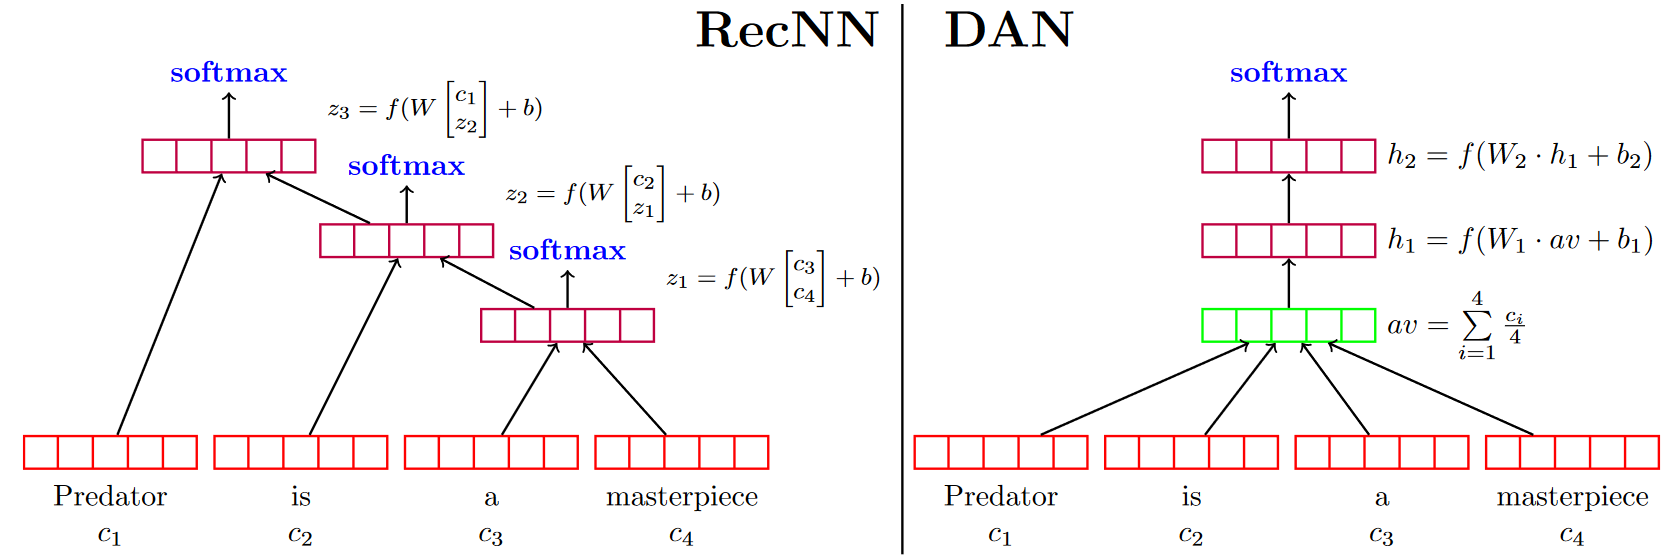
\includegraphics[width=15cm]{img/rnn_dan}
	\end{center}
	%légende de l'image
	\caption{Comparison of the DAN model system with a basic RNN\cite{dan_1}\label{fig:1}}
\end{figure} 

\section{Improving Performances}
To improve the performance of DAN network we have used we can perform dropout on input word sequences by randomly dropping a word in a sentence by a some defined probability. The basic motto of dropout is that it prevents overfitting of the data in the model, by randomly removing part of the data, thus artificially increasing the number of different examples.
In DAN model we can drop word tokens or part of the embedding average. Using this method our input sequence to the model see different token sequence for each input X. However, dropout may also drop words or characters which are really necessary for  the analysis of the input sequence. But most of time this method improves the performance of the model.
We can note that the dropout technique work well with DAN models although it can alter and deteriorate the results if applied to other models like RNN or LSTM.

\section{DAN For Predictive Maintenance}
In our project we are using the DAN model to predict the next occurring system log in a sequence of many logs. As described in the upcoming sections, we have a very large data set (comparatively to the usual datasets used in deep learning). Compared with other state of the art architectures like the RNN or LSTM, which concentrate on achieving high performance with a low amount of data, the DAN would give us equivalent or better performance, while maintaining a very low training time necessary to draw the most of the amount of available data.
DAN can also magnify small and meaningful differences from the different logs. Another interesting feature of, the DAN is its ability to incorporate out-of-domain data which is useful to maintain a stable predictive ability.
